\documentclass[preview]{standalone}
\usepackage{tikz}
\begin{document}
  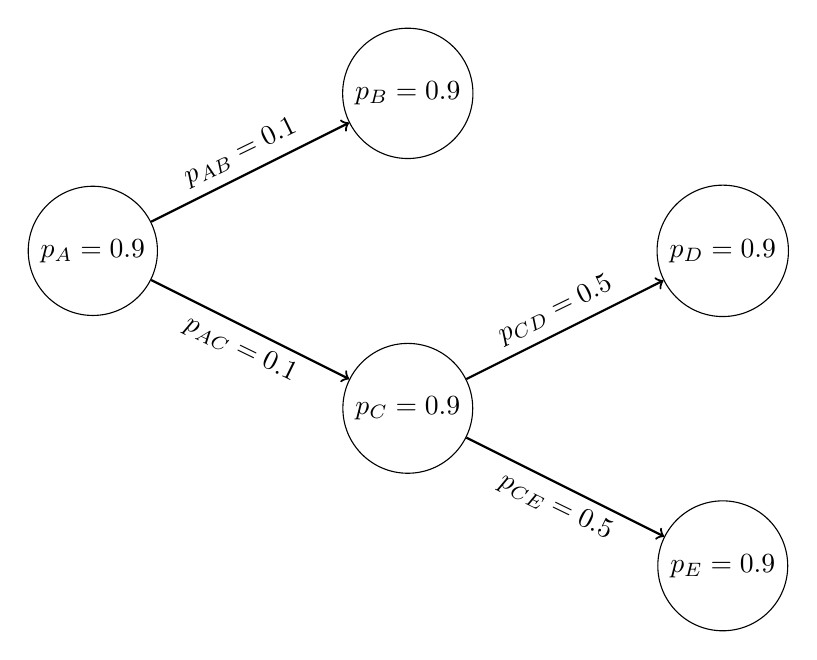
\begin{tikzpicture}[
roundnode/.style={circle, draw=black, minimum size=7mm},
]
%Nodes
\node[roundnode]      at (0,0) (nodeA) {$p_A=0.9$};
\node[roundnode]      at (4,2) (nodeB) {$p_B=0.9$};
\node[roundnode]      at (4,-2) (nodeC) {$p_C=0.9$};
\node[roundnode]      at (8,-0) (nodeD) {$p_D=0.9$};
\node[roundnode]      at (8,-4) (nodeE) {$p_E=0.9$};
%Lines
\path[->,draw,thick] (nodeA) edge node[above, rotate=26] {$p_{AB}=0.1$}(nodeB) ;
\path[->,draw,thick] (nodeA) edge node[below, rotate=334] {$p_{AC}=0.1$}(nodeC) ;
\path[->,draw,thick] (nodeC) edge node[above, rotate=26] {$p_{CD}=0.5$}(nodeD) ;
\path[->,draw,thick] (nodeC) edge node[below, rotate=334] {$p_{CE}=0.5$}(nodeE);
\end{tikzpicture}
\end{document}

% convert -density 300 riskModel.pdf -quality 90 riskModel.png
